% Section content template for individual Educative lessons
% This file contains the actual content for a specific section
% Generated from Educative API section content

% Section: Getting Ready: Stack Overflow
% Section ID: 5007773721165824
% Section Slug: getting-ready-stack-overflow
% Generated: 2025-12-12T22:48:52.487799

\subsection{Problem definition}\label{raksgJKDta6LUku0_v0OK-1}
\\
\textbf{Stack Overflow} is a Q\&A website for programmers and developers, irrespective of their expertise level in the domain. It has a wide variety of questions on computer science and programming topics. Registered users can post new questions and answer questions from other users. Each user can collect reputation points. These points are affected by the upvotes or downvotes received by the user on their questions or answers. More reputation points allow users to perform additional functions, like voting to close or delete a question. On achieving reputation milestones, users are awarded badges to highlight their credibility.

\begin{figure}[htbp]
 \centering
 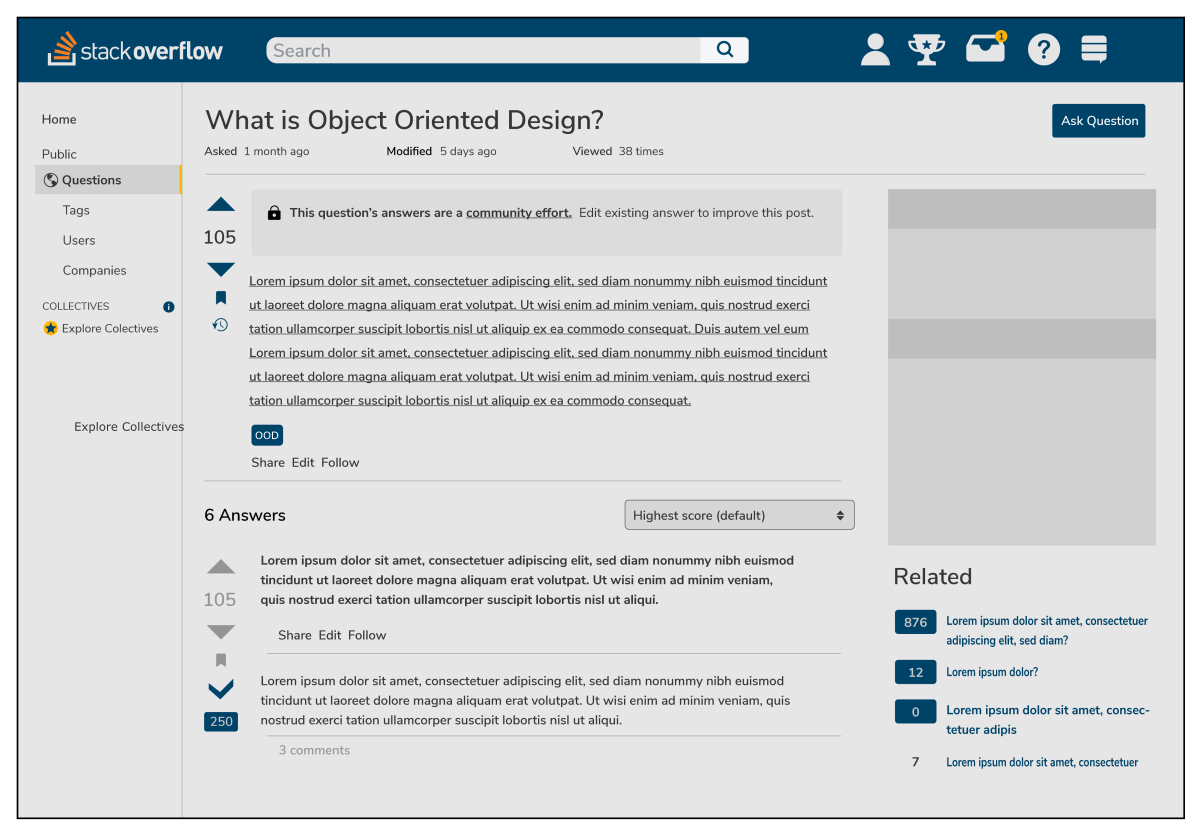
\includegraphics[width=0.5\textwidth]{Images/chapter_20/section_5007773721165824/6333432031215616.png}
 \caption{A question page on Stack Overflow}
\end{figure}

\subsection{Expectations from the interviewee}\label{raksgJKDta6LUku0_v0OK-2}
\\
It is important to narrow down the components to be included in your Stack Overflow design. The following section provides an overview of some of the main expectations that the interviewer will want to hear you discuss in more detail during the interview:

\subsubsection{Discoverability}\label{QwphTDLN2N-L8SKK6HEPW}
\\
You may want to ask the interviewer the following to get a better understanding of how Stack Overflow's discoverability works:

\begin{itemize}
\item
\protect\phantomsection\label{NjKaAJcJ9_MIX9Lm0wuN_}
How are users able to search for questions?
\item
\protect\phantomsection\label{JS1NLpiyKJy4Wr9YoYW2b}
Is there a way to filter questions using tags or users?
\end{itemize}

\subsubsection{Reputation}\label{7w9wz8d3z3SrYaignOMM2}
\\
Reputation points affect user privileges. Therefore, it's important to ask the interviewer the following questions about reputation points:

\begin{itemize}
\item
How are reputation points calculated? Do users get points for asking or answering questions?
\item
How many points are required for users to get moderator access?
\end{itemize}

\subsubsection{Voting}\label{K-LK1TR9AJoexdLA30XCE}
\\
Voting is one of the main features of Stack Overflow. It gives insight into which questions or answers are more popular among users. Make sure to ask the following questions to understand how voting works in Stack Overflow:

\begin{itemize}
\item
\protect\phantomsection\label{RuNzA7aMck_w9R_hNbdiT}
What are the different types of voting allowed on Stack Overflow? Are you allowed to upvote and downvote?
\item
\protect\phantomsection\label{-yoZuSIKK-wtwDp6WioQW}
How does voting work when a question has to be closed and deleted? Which user can vote in such circumstances?
\end{itemize}

\subsubsection{Bounty}\label{y4RSc0MQ3ARuKSoGPKUc_}
\\
\textbf{Bounty} is a special reputation placed on a question that is not being noticed or answered. Any user who answers a bounty question receives reputation points equal to the bounty value. You need to clarify the bounty requirements from the interviewer by asking the following questions:

\begin{itemize}
\item
\protect\phantomsection\label{LmibANtZf6dkKQB-U8r9p}
How are reputation points awarded on bounty questions?
\item
\protect\phantomsection\label{0VqQifyO4jggAOlUsDhFZ}
When do users start a bounty? How long does a bounty last before expiring?
\end{itemize}

\subsection{Design approach}\label{CO1fw12Xo70xkjutOggV4}
\\
We'll design Stack Overflow using the bottom-up design approach. For this purpose, we'll follow the steps below:

\begin{itemize}
\item
\protect\phantomsection\label{ByYcv-pn7JeASQylc14uB}
Identify and design the smallest components first, like a question and an answer.
\item
\protect\phantomsection\label{AvLb9h3XA4DF8t5lzMuWV}
Use these small components to design additional components, for example, comments, bounty, and tags.
\item
\protect\phantomsection\label{rnv70plguM8-4gFNgLDjh}
Repeat the steps above until we design the complete Stack Overflow platform.
\end{itemize}

\subsection{Design pattern~}\label{wYLoSVzV9FNni3Zr6G0Ou}
\\
During an interview, discussing the design patterns that Stack Overflow falls under is always a good practice. Stating the design patterns gives the interviewer a positive impression and shows that the interviewee is well-versed in the advanced concepts of object-oriented design.
\\
Try to answer the following question. If you are not familiar with design patterns, don't worry! You can learn about them by asking, ``Define design patterns.''

\textbf{Question:}

Which design pattern(s) should be used to design Stack Overflow? Please elaborate on your choice(s).

Let's explore the requirements of Stack Overflow in the next lesson.

% End of section content